\documentclass{beamer}
\usepackage{amsmath}
\usepackage{hyperref}
\usepackage{listings}
\usepackage{xcolor}
\hypersetup{colorlinks=true, citecolor=blue, filecolor=blue, linkcolor=blue, urlcolor=blue}
\definecolor{codegreen}{rgb}{0,0.6,0}
\definecolor{codegray}{rgb}{0.5,0.5,0.5}
\definecolor{codepurple}{rgb}{0.58,0,0.82}
\definecolor{backcolour}{rgb}{0.95,0.95,0.92}
 
\lstdefinestyle{mystyle}{
    backgroundcolor=\color{backcolour},   
    commentstyle=\color{codegreen},
    keywordstyle=\color{magenta},
    numberstyle=\tiny\color{codegray},
    stringstyle=\color{codepurple},
    basicstyle=\ttfamily\footnotesize,
    breakatwhitespace=false,         
    breaklines=true,                 
    captionpos=b,                    
    keepspaces=true,                 
    %numbers=left,                    
    numbersep=5pt,                  
    showspaces=false,                
    showstringspaces=false,
    showtabs=false,                  
    tabsize=2
}
 
\lstset{style=mystyle}

\mode<presentation> {

% The Beamer class comes with a number of default slide themes
% which change the colors and layouts of slides. Below this is a list
% of all the themes, uncomment each in turn to see what they look like.

%\usetheme{default}
\usetheme{AnnArbor}
%\usetheme{Antibes}
%\usetheme{Bergen}
%\usetheme{Berkeley}
%\usetheme{Berlin}
%\usetheme{Boadilla}
%\usetheme{CambridgeUS}
%\usetheme{Copenhagen}
%\usetheme{Darmstadt}
%\usetheme{Dresden}
%\usetheme{Frankfurt}
%\usetheme{Goettingen}
%\usetheme{Hannover}
%\usetheme{Ilmenau}
%\usetheme{JuanLesPins}
%\usetheme{Luebeck}
%\usetheme{Madrid}
%\usetheme{Malmoe}
%\usetheme{Marburg}
%\usetheme{Montpellier}
%\usetheme{PaloAlto}
%\usetheme{Pittsburgh}
%\usetheme{Rochester}
%\usetheme{Singapore}
%\usetheme{Szeged}
%\usetheme{Warsaw}

% As well as themes, the Beamer class has a number of color themes
% for any slide theme. Uncomment each of these in turn to see how it
% changes the colors of your current slide theme.

%\usecolortheme{albatross}
%\usecolortheme{beaver}
%\usecolortheme{beetle}
%\usecolortheme{crane}
%\usecolortheme{dolphin}
%\usecolortheme{dove}
%\usecolortheme{fly}
%\usecolortheme{lily}
%\usecolortheme{orchid}
%\usecolortheme{rose}
%\usecolortheme{seagull}
%\usecolortheme{seahorse}
%\usecolortheme{whale}
%\usecolortheme{wolverine}

%\setbeamertemplate{footline} % To remove the footer line in all slides uncomment this line
\setbeamertemplate{footline}[page number] % To replace the footer line in all slides with a simple slide count uncomment this line

\setbeamertemplate{navigation symbols}{} % To remove the navigation symbols from the bottom of all slides uncomment this line
}

\usepackage{graphicx} % Allows including images
\usepackage{booktabs} % Allows the use of \toprule, \midrule and \bottomrule in tables
%\usepackage {tikz}
\usepackage{tkz-graph}
\GraphInit[vstyle = Shade]
\tikzset{
  LabelStyle/.style = { rectangle, rounded corners, draw,
                        minimum width = 2em, fill = yellow!50,
                        text = red, font = \bfseries },
  VertexStyle/.append style = { inner sep=5pt,
                                font = \normalsize\bfseries},
  EdgeStyle/.append style = {->, bend left} }
\usetikzlibrary {positioning}
%\usepackage {xcolor}
\definecolor {processblue}{cmyk}{0.96,0,0,0}
%----------------------------------------------------------------------------------------
%	TITLE PAGE
%----------------------------------------------------------------------------------------

\title[Constrained Optimization]{Numerical Optimization 15: Constrained Optimization} %

\author{Qiang Zhu} % Your name
\institute[University of Nevada Las Vegas] % Your institution as it will appear on the bottom of every slide, may be shorthand to save space
{
University of Nevada Las Vegas\\ % Your institution for the title page
\medskip
}
\date{\today} % Date, can be changed to a custom date

\begin{document}

\begin{frame}
\titlepage % Print the title page as the first slide
\end{frame}

\begin{frame}
\frametitle{Overview} % Table of contents slide, comment this block out to remove it
\tableofcontents % Throughout your presentation, if you choose to use \section{} and \subsection{} commands, these will automatically be printed on this slide as an overview of your presentation
\end{frame}

%----------------------------------------------------------------------------------------
%	PRESENTATION SLIDES
%----------------------------------------------------------------------------------------

%------------------------------------------------

\section{Constrained Optimization}
\begin{frame}{Noisy Descent}
Fitting Surrogate Models
\begin{figure}
\centering
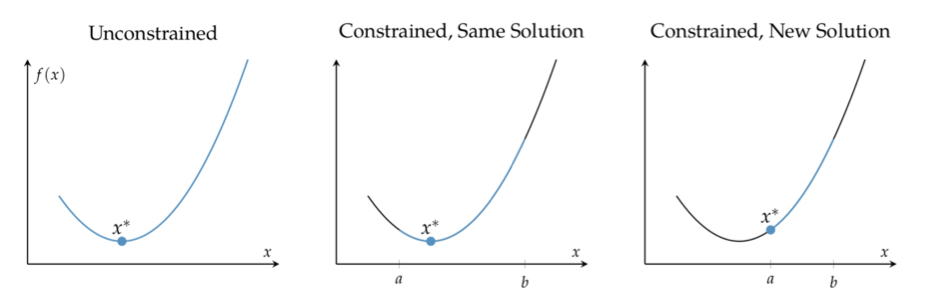
\includegraphics[width=120mm]{Figs/constraint-ab.jpeg}
\end{figure}   

\end{frame}

\section{Constraints}
\begin{frame}{Constraints}
Constraints are not typically specified directly through a known feasible set X . Instead, the feasible set is typically formed from two types of constraints:

\begin{itemize}
    \item equality constraints, $h(x)=0$ 
    \item inequality constraints, $g(x) \leq 0$
    
\end{itemize}

Any optimization problem can be rewritten using these constraints
\begin{gather*}
    ~~~~~ \underset{\boldsymbol{x}}{\min} ~ f(\boldsymbol{x})\\
    {s.t.}~~~~ h_i(x) = 0 \\
    ~~~~~~~~~ g_j(x) = 0
\end{gather*}

\end{frame}

\section{Transformations to Remove Constraints}
\begin{frame}{Transformations to Remove Constraints}
In some cases, it may be possible to transform a problem so that constraints can be removed. For example, bound constraints a ≤ x ≤ b can be removed by passing x through a transform

\begin{equation*}
x = \frac{b+a}{2} + \frac{b-a}{2}\bigg(\frac{2\hat{x}}{1+\hat{x}^2}\bigg)
\end{equation*}

Below is an example
\begin{gather*}
    ~~~~~ \underset{x}{\min} ~ x\sin{x}\\
    {s.t.}~~~~ 2\leq x \leq 6 \\
\end{gather*}
Can be transformed to 
\begin{gather*}
    \underset{\hat{x}}{\min} ~ \bigg[4+2\bigg(\frac{2\hat{x}}{1+\hat{x}^2}\bigg)x
    + \sin \bigg[ 4 + 2\frac{2\hat{x}}{1+\hat{x}^2}\bigg]
\end{gather*}

\end{frame}

\section{Lagrange Multipliers}
\begin{frame}{Lagrange Multipliers}
The method of Lagrange multipliers is used to optimize a function subject to equality
constraints. 
\begin{gather*}
    ~~~~~ \underset{\boldsymbol{x}}{\min} ~ f(\boldsymbol{x})\\
    {s.t.}~~~~ h_i(x) = 0 
\end{gather*}

where $f$ and $h$ have continuous partial derivatives.

We can formulate the Lagrangian, which is a function of the design variables,
\begin{gather*}
    \mathcal{L}(x, \lambda) = f(x) - \lambda h(x) 
\end{gather*}

Solving $\nabla \mathcal{L}(x, \lambda)$ = 0. Specifically, $\nabla_x \mathcal{L}$ = 0 gives us the condition $\nabla f= \lambda \nabla h$, and $\nabla \lambda \mathcal{L}=0$ gives us $h(x)=0$. Any solution is considered a critical point.

\end{frame}

\begin{frame}{Lagrange Multipliers to a single equality condition}
The method of Lagrange multipliers is used to optimize a function subject to equality
constraints. 
\begin{gather*}
    ~~~~~ \underset{\boldsymbol{x}}{\min} ~ -\exp[-(x_1x_2-3/2)^2 - (x_2-3/2)^2] \\
    {s.t.}~~~~~~~~~~~~~~~~~~~~~~~~~~~~~~~~~ x_1 - x_2^2 = 0 
\end{gather*}

We can formulate the Lagrangian, 
\begin{equation*}
    \mathcal{L}(x, \lambda) = -\exp[-(x_1x_2-3/2)^2 - (x_2-3/2)^2] + \lambda(x_1 - x_2^2)
\end{equation*}
We compute
\begin{itemize}
    \item $\frac{\partial \mathcal{L}}{\partial x_1}$
    \item $\frac{\partial \mathcal{L}}{\partial x_2}$
    \item $\frac{\partial \mathcal{L}}{\partial \lambda}$
\end{itemize}

\end{frame}


\begin{frame}{Lagrange Multipliers to multiple equality conditions}
The method of Lagrange multipliers is used to optimize a function subject to equality
constraints. 
\begin{gather*}
    ~~~~~ \underset{\boldsymbol{x}}{\min} ~ -\exp[-(x_1x_2-3/2)^2 - (x_2-3/2)^2] \\
    {s.t.}~~~~~~~~~~~~~~~~~~~~~~~~~~~~~~~~~ x_1 - x_2^2 = 0 
\end{gather*}

We can formulate the Lagrangian, 
\begin{equation*}
    \mathcal{L}(x, \lambda) = -\exp[-(x_1x_2-3/2)^2 - (x_2-3/2)^2] + \lambda(x_1 - x_2^2)
\end{equation*}
We compute
\begin{itemize}
    \item $\frac{\partial \mathcal{L}}{\partial x_1}$
    \item $\frac{\partial \mathcal{L}}{\partial x_2}$
    \item $\frac{\partial \mathcal{L}}{\partial \lambda}$
\end{itemize}

\end{frame}

\section{Summary}
\begin{frame}{Summary}
    \begin{itemize}
        \item Constraints are requirements on the design points that a solution must satisfy.
        \item Some constraints can be transformed or substituted into the problem to result in an unconstrained optimization problem.
        \item Analytical methods using Lagrange multipliers yield the generalized Lagrangian and the necessary conditions for optimality under constraints.
        \item A constrained optimization problem has a dual problem formulation that is easier to solve and whose solution is a lower bound of the solution to the original problem.
    \end{itemize}
\end{frame}
\end{document}

